%!TEX encoding = UTF-8 Unicode
%
% Laboratorio di Fisica III
% Esperienza 11
% Anno accademico 2013/2014
% Daniele Brugnara, Alessandro Casalino
%

\documentclass {article}
\usepackage[utf8]{inputenc}
\usepackage{fontenc}
\usepackage[english]{babel}
\usepackage{graphicx}
\usepackage{float}
\usepackage{fancyhdr}
\usepackage{listingsutf8}
\usepackage{xcolor}
\usepackage{amsfonts}
\usepackage{amsmath}
\usepackage{amssymb}	
\usepackage{wrapfig}
\usepackage{enumitem}
\usepackage{subfigure}
\usepackage{amssymb}
\usepackage{amsmath}
\usepackage [a4paper, top=2.5cm, bottom=2cm, left=1.5cm, right=1.5cm] {geometry}
\pagestyle{fancy}

% cambiato bottom da 1.8 + logo

\makeatletter
\@addtoreset{section}{part}
\makeatother
\rhead{\LARGE Project 1}

\lhead{\large Numerically solving a differential equation}
\lfoot{D. Brugnara, M. Seclì}
\cfoot{}
\rfoot{\thepage}
\renewcommand{\headrulewidth}{0.7pt}
\renewcommand{\footrulewidth}{0.7pt}

\definecolor{dkgreen}{rgb}{0,0.6,0}
\definecolor{dred}{rgb}{0.545,0,0}
\definecolor{dblue}{rgb}{0,0,0.545}
\definecolor{lgrey}{rgb}{0.9,0.9,0.9}
\definecolor{gray}{rgb}{0.4,0.4,0.4}
\definecolor{darkblue}{rgb}{0.0,0.0,0.6}
\lstdefinelanguage{cpp}{
      backgroundcolor=\color{lgrey},  
      basicstyle=\footnotesize \ttfamily \color{black} \bfseries,   
      breakatwhitespace=false,       
      breaklines=true,               
      captionpos=b,                   
      commentstyle=\color{dkgreen},   
      deletekeywords={...},          
      escapeinside={\%*}{*)},                  
      frame=single,                  
      language=C++,                
      keywordstyle=\color{purple},  
      morekeywords={BRIEFDescriptorConfig,string,TiXmlNode,DetectorDescriptorConfigContainer,istringstream,cerr,exit}, 
      identifierstyle=\color{black},
      stringstyle=\color{blue},      
      numbers=right,                 
      numbersep=5pt,                  
      numberstyle=\tiny\color{black}, 
      rulecolor=\color{black},        
      showspaces=false,               
      showstringspaces=false,        
      showtabs=false,                
      stepnumber=1,                   
      tabsize=5,                     
      title=\lstname,                 
    }

\begin{document}

\section{\LARGE Numerically solving a differential equation through a linear system}

\subsection{Abstract}

In this project we aim to solve a special kind of differential equation using a numerical procedure that allows us to express the equation through a linear system. We will study some algorithms to solve such a problem, focusing on the efficiency of the program, setting our goal more on speed than generality. 

The differential equation we're interested in studying is of the type

\begin{equation}
	u''(x)= - f(x)
	\label{differential_eq}
\end{equation}

In our case we will limit our solutions using the contour conditions of $u(0)=0$ and $u(L)=0$, where $[0, L]$ is our domain of integration.
Using Taylor expansion it is possible to express the second derivative of a function $u(x)$ as

\begin{equation}
	u''(x)= \frac{u(x-h)-2 u(x)+u(x+h)}{h^2}+ \O (h^2)
\end{equation}

We are therefore able to discretize equaition (\ref{differential_eq}) using $N$ points, obtaining:

$$u''_i= \frac{u_{i-1}-2 u_i+u_{i+1}}{h^2}=-f_i \quad \quad i \in \left\lbrace 1 \cdots N\right\rbrace$$

Using the matrix representation, we can write equation (\ref{differential_eq}) as

\begin{equation}
 \begin{pmatrix}
   2 & -1 &  0 & 0 & \cdots & 0  \\
  -1 &  2 & -1 & 0 & \cdots & 0  \\
   0 &-1 &  2 & -1 & \cdots & 0 \\
  \vdots  & \vdots  & & \ddots & & \vdots   \\
   0 &  0 & \cdots  & -1 & 2 & -1 \\
   0 &  0 & \cdots & \cdots  & -1 & 2
 \end{pmatrix}
 \begin{pmatrix}
  u_0 \\
  u_1 \\
  u_2 \\
  \vdots  \\
  u_{N-2} \\
  u_{N-1} 
 \end{pmatrix}
 = h^2
 \begin{pmatrix}
  f_0 \\
  f_1 \\
  f_2 \\
  \vdots  \\
  f_{N-2} \\
  f_{N-1} 
 \end{pmatrix}
\end{equation}

Note how, with this system it is already implied that $f(0)=0$ e $f(L)=0$, since the first and last equations state that

$$h^2 f_0=\frac{2 u_0-u_1}{h^2}=\frac{-1 u_{-1}+2 u_0-u_1}{h^2}$$

$$h^2 f_{N-1}=\frac{-u_{N-2}+2 u_{N-1}}{h^2}=\frac{-u_{N-2}+2 u_{N-1}-u_N}{h^2}$$ 

Since the boundary conditions of the differential equations state that $u_{-1}=u(0)=0$ and $u_{N}=u(L)=0$.  

This linear system is indeed very particular and has a clear pattern. We will first focus on finding a solving algorithm for a general tridiagonal matrix and after we will try to implement another program to solve this particular system with the intent of lowering the number of calculation and therefore the computation time.

\subsection{General algorithm for solving a tridiagonal matrix through back and forward substitution}

A general tridiagonal system can be expressed as

\begin{equation}
 \begin{pmatrix}
   b_0 & c_0 &  0 & 0 & \cdots & 0  \\
  a_1 & b_1 & c_1 & 0 & \cdots & 0  \\
   0 & a_2 &  b_2 & c_2 & \cdots & 0 \\
  \vdots  & \vdots  & & \ddots & & \vdots   \\
   0 &  0 & \cdots  & a_{N-2} & b_{N-2} & c_{N-2} \\
   0 &  0 & \cdots & \cdots  & a_{N-1} & b_{N-1}
 \end{pmatrix}
 \begin{pmatrix}
  u_0 \\
  u_1 \\
  u_2 \\
  \vdots  \\
  u_{N-2} \\
  u_{N-1} 
 \end{pmatrix}
 =h^2
 \begin{pmatrix}
  f_0 \\
  f_1 \\
  f_2 \\
  \vdots  \\
  f_{N-2} \\
  f_{N-1} 
 \end{pmatrix}
\end{equation}

We will describe the algorithm we used for this system first for a 3x3 tridiagonal matrix, and after we will demonstrare its validity for a square tridiagonal matrix of optional dimension.
\\
\\
\\
\\
\\
MATRIX 3X3:

\begin{equation}
\left(
\begin{array}{ccc|c}
   b & c &  0 & f_0 \\
   a & b &  c & f_1 \\
   0 & a &  b & f_2 \\
\end{array}	
\right)
\longrightarrow
\end{equation}
\begin{equation}
Passage 1:
\left(
\begin{array}{ccc|c}
   1 & c/b & 0 & f_0/b \\
   a & b & c & f_1 \\
   0 & a & b & f_2 \\
\end{array}
\right)
\longrightarrow\\
\end{equation}
\begin{equation}
Passage 2:
\left(
\begin{array}{ccc|c}
  1 & c/b & 0 & f_0/b \\
  0 & \frac{b-(c/b)a)}{b-(c/b)a} & \frac{c}{(b-(c/b)a} & \frac{f_1-af_0}{b-(c/b)a} \\
  0 & 0 & \frac{b-\frac{ac}{b-ac/b}}{b-\frac{ac}{b-ac/b}} & \frac{f_2-af_1}{b-\frac{ac}{b-ac/b}} \\ 
\end{array}
\right)
=
\left(
\begin{array}{ccc|c}
  1 & c/b & 0 & f_0/b \\
  0 & 1 & \frac{c}{b-ac/b} & \frac{f_1-af_0}{b-(c/b)a} \\
  0 & 0 & 1 & \frac{f_2-af_1}{b-\frac{ac}{b-ac/b}} \\ 
\end{array}
\right)
\longrightarrow\\\
\end{equation}
\begin{equation}
Passage 3:
\left(
\begin{array}{ccc|c}
  1 & 0 & 0 & f_0/b-f_1(c/b) \\
  0 & 1 & 0 & \frac{f_1-af_0}{b-(c/b)a}-f_2\frac{c}{b-ac/b} \\
  0 & 0 & 1 & \frac{f_2-af_1}{b-\frac{ac}{b-ac/b}} \\
\end{array}
\right)
\end{equation}

Now it's very simple to solve the system.
\\
\\
\\
MATRIX (n+1)x(n+1)

Before starting to demonstrate that the above passages can be done also for a (n+1)x(n+1) matrix, supposed that they work for a nxn one, we can notice that, in general, for a square matrix of optional dimension N, doing the passage 2 until the penultime row we obtain:

$$A_{N-1,N}=\frac{c}{bet(N-1)}$$
where 
$$bet(n)=b_0-\frac{ac}{b_1-\frac{ac}{b_2-\frac{ac}{\frac{\cdots}{b_{n-1}-\frac{ac}{b_n}}}}}$$
(here all the $b_i's$ have the same value; the index i helps only to count them).

Now we do the passage 2 until the last row (we focus only on the tridiagonal matrix; if we manage to obtain the unitary matrix the system is solved); we obtain:

\begin{equation}
\left(
\begin{array}{ccccc}
  1 & c/b & 0 & 0 & \cdots \\
  0 & 1 & fract{c}{b-ac/b} & 0 & \cdots \\
  \cdots & \cdots & \cdots & \cdots & \cdots \\
  \cdots & \cdots & \cdots & 1 & c/bet(n) \\
  \cdots & \cdots & \cdots & 0 & 1 \\
\end{array}
\right)
\end{equation}
and simply subtracting, from the n-row, the (n+1)-row multiplied for bet(n)/c:
\begin{equation}
\left(
\begin{array}{ccccc}
  1 & c/b & 0 & 0 & \cdots \\
  0 & 1 & \frac{c}{b-ac/b} & 0 & \cdots \\
  \cdots & \cdots & \cdots & \cdots & \cdots \\
  \cdots & \cdots & \cdots & 1 & 0 \\
  \cdots & \cdots & \cdots & 0 & 1 \\
\end{array}
\right)
\end{equation}

Now, ignoring the (n+1)-row and the (n+1)-column, we have a nxn matrix which we can bring back to the identity going on with the passage 3.
\\
\\
\\
ALGORITHM IN C++

Translating the above algorithm in C++ language and working only on the vector f and on the solution vector u, we obtain the following code:

\begin{lstlisting}[language=cpp]
	u[0]=f[0]/(bet=b);
    for(int j = 1; j < N; j++) {
        gam[j]=c/bet;
        bet=b-a*gam[j];
        u[j]=(f[j]-a*u[j-1])/bet;
    }
    for (int j = (N-2); j >= 0; j--) u[j] -= gam[j+1]*u[j+1];
\end{lstlisting}

\subsection{Particular algorithm}

Using the regular Gaussian elimination algorithm we proceed to find a specific solution of our system as follows; we will start form a 3x3 matrix as before, and then demonstrate it for a matrix of optional dimension.
\\
\\
\\
\\
\\
MATRIX 3X3:

\begin{equation}
\left(
\begin{array}{ccc|c}
   2 & -1 & 0 & f_0 \\
   -1 & 2 & -1 & f_1 \\
   0 & -1 & 2 & f_2 \\
\end{array}	
\right)
\longrightarrow
\end{equation}
\begin{equation}
Passage 1:
\left(
\begin{array}{ccc|c}
   2 & -1 & 0 & f_0 \\
   0 & 3 & -2 & f_1(1+1)+f_0 \\
   0 & 0 & 4 & f_2(2+1)+f_1 \\
\end{array}
\right)
\end{equation}
that is: $a_{i,j} \rightarrow (i+1)a_{i,j}+a{i-1,j}$ for i going from 1 to (n-1), where n is the matrix's dimension (3 in this case)
\begin{equation}
\longrightarrow\\
Passage 2:
\left(
\begin{array}{ccc|c}
  2 & -1 & 0 & f_0 \\
  0 & 3 & -1 & f_1(1+1)+f_0 \\
  0 & 0 & 1 & \frac{f_2}{3+1}\\ 
\end{array}
\right)
\end{equation}
that is: $a_{n-1, j} \rightarrow \frac{a{n-1,j}}{n+1}$ where n is the matrix's dimension
\begin{equation}
Passage 3:
\longrightarrow\\
\left(
\begin{array}{ccc|c}
  1 & 0 & 0 & \frac{f_0+(0+1)f_1}{0+2} \\
  0 & 1 & 0 & \frac{f_1+(1+1)f_2}{1+2} \\
  0 & 0 & 1 & \frac{f_2}{3+1} \\
\end{array}
\right)
\end{equation}
that is $a_{i,j} \rightarrow \frac{a_{i,j}+(i+1)a_{i+1,j}}{i+2}$ for i going from 0 to (n-1)
\\
Now it's very simple to solve the system.
\\
\\
\\
MATRIX (n+1)x(n+1)

We focus only on the tridiagonal matrix and try to obtain the unitary matrix; to do this let's to passage 1 until the n+1 row.

\begin{equation}
\left(
\begin{array}{ccccc}
  2 & -1 & 0 & 0 & \cdots \\
  0 & 3 & -2 & 0 & \cdots \\
  \cdots & \cdots & \cdots & \cdots & \cdots \\
  \cdots & \cdots & \cdots & n+2 & -(n+1) \\
  \cdots & \cdots & \cdots & -1 & 2 \\
\end{array}
\right)
\end{equation}
and simply subtracting, from the n-row, the (n+1)-row multiplied for bet(n)/c:
\begin{equation}
\left(
\begin{array}{ccccc}
  1 & c/b & 0 & 0 & \cdots \\
  0 & 1 & \frac{c}{b-ac/b} & 0 & \cdots \\
  \cdots & \cdots & \cdots & \cdots & \cdots \\
  \cdots & \cdots & \cdots & 1 & 0 \\
  \cdots & \cdots & \cdots & 0 & 1 \\
\end{array}
\right)
\end{equation}

Now, ignoring the (n+1)-row and the (n+1)-column, we have a nxn matrix which we can bring back to the identity going on with the passage 3.
\\
\\
\\
ALGORITHM IN C++

Translating the above algorithm in C++ language and working only on the vector f and on the solution vector u, we obtain the following code:

\begin{lstlisting}[language=cpp]
	u[0]=f[0]/(bet=b);
    for(int j = 1; j < N; j++) {
        gam[j]=c/bet;
        bet=b-a*gam[j];
        u[j]=(f[j]-a*u[j-1])/bet;
    }
    for (int j = (N-2); j >= 0; j--) u[j] -= gam[j+1]*u[j+1];
\end{lstlisting}
\subsection{Errors}



\subsection{Time}

\begin{figure}[ht]
 \centering
   {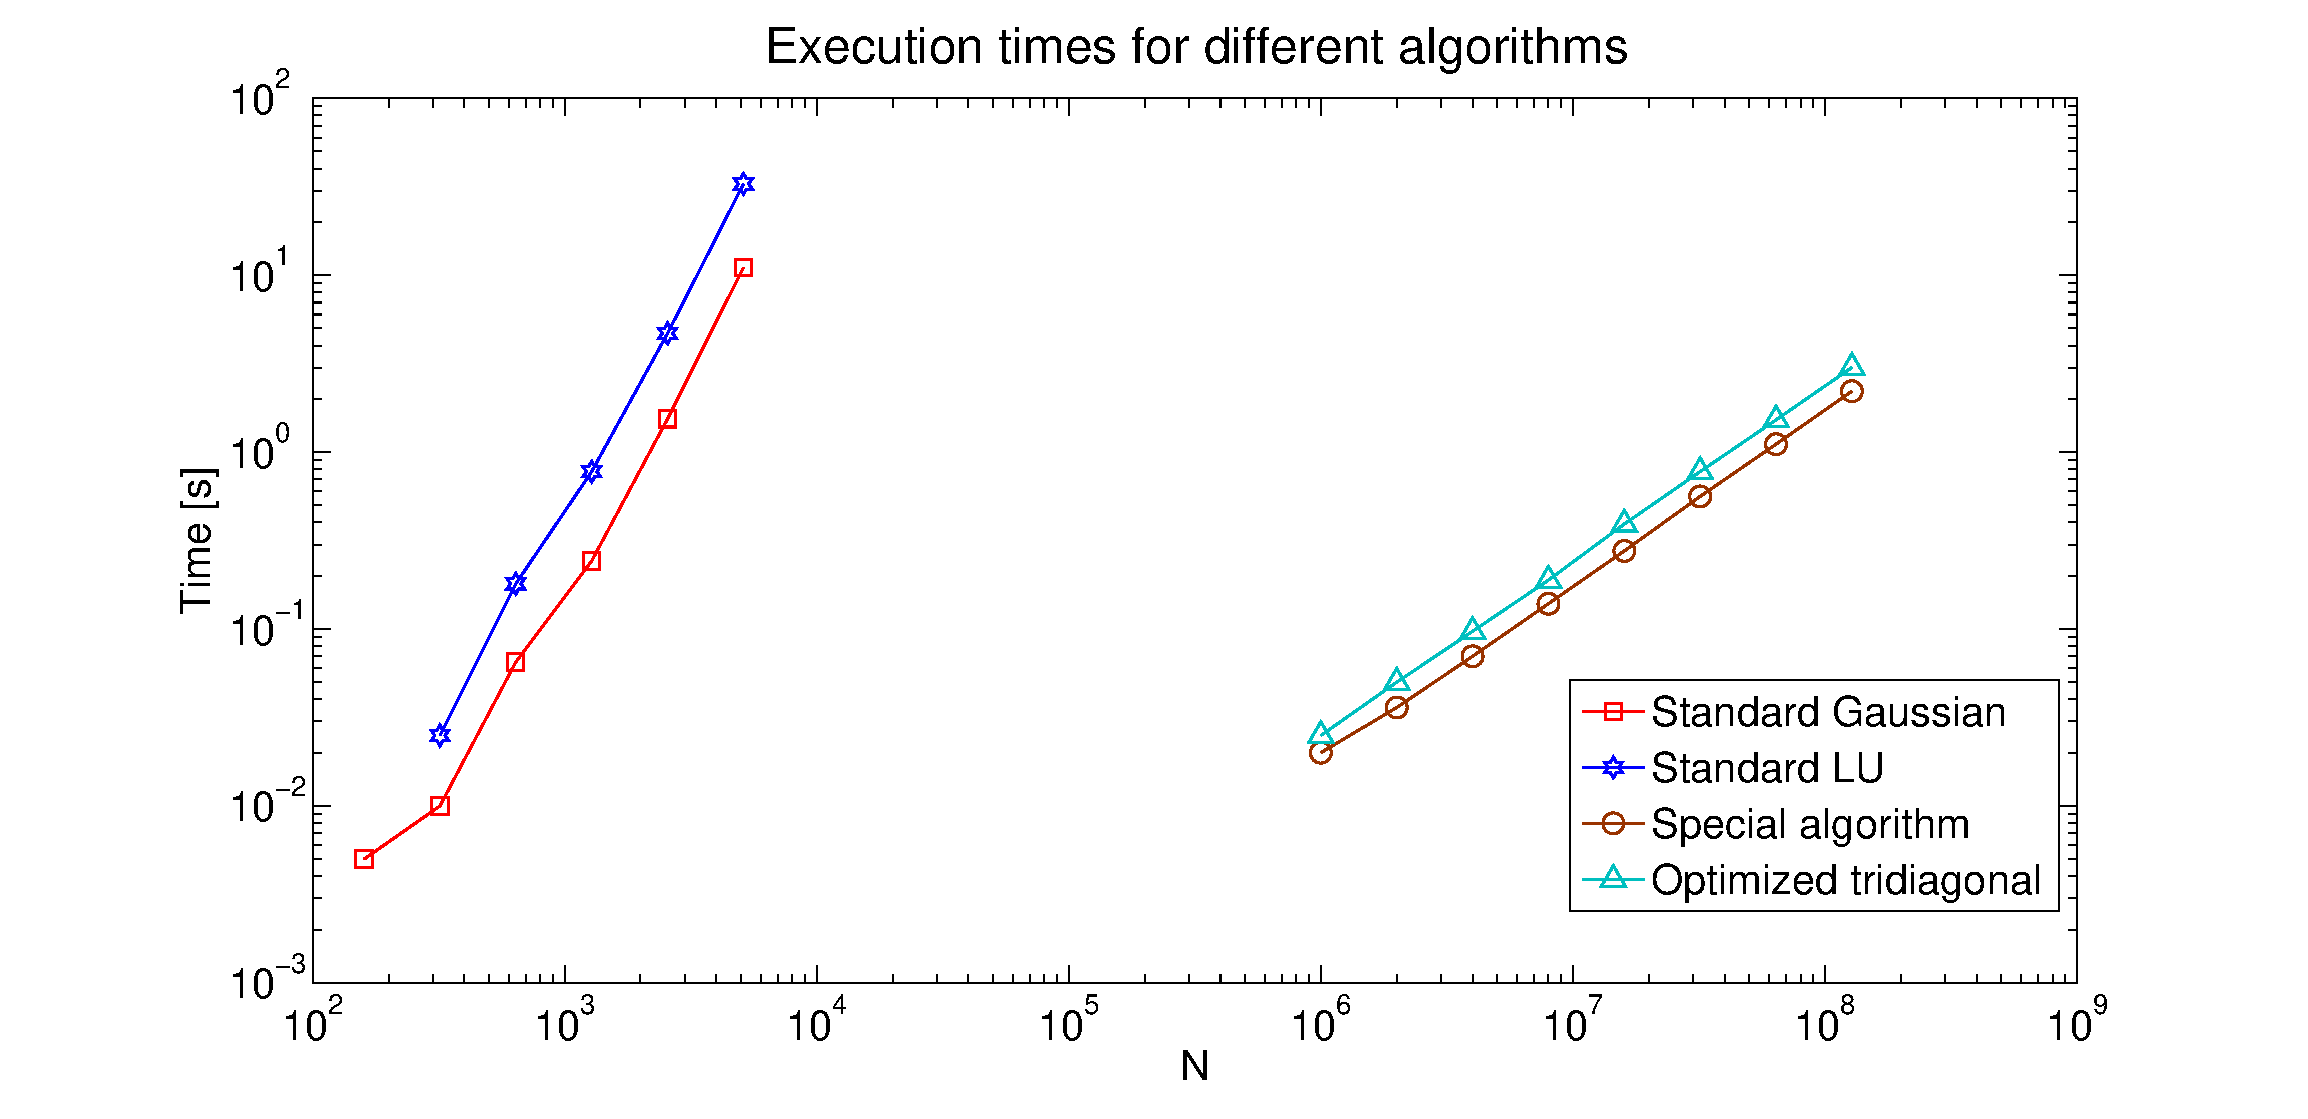
\includegraphics[width=12cm]{times.eps}}
 \caption{***}
\end{figure}


\end{document}